\chapter{Wind stress plus heating}
\label{chapter:winds_and_heating}

In this chapter, we document a test configured with a constant zonal
wind stress
\begin{equation}
 \bftau  =  (0.1, 0)~\mbox{N}~\mbox{m}^{-2}
\end{equation}
plus a constant positive heat flux applied in the top grid cell
\begin{equation}
Q=100~\mbox{W}~\mbox{m}^{-2}.
\end{equation}
The temperature is initialized with uniform value of
$15^{\circ}~\mbox{C}$.  In this experiment, the positive buoyancy
applied to the surface grid cell is mixed downward by the mechanical
forcing by wind stress.  This process develops a nonzero
stratification at depth, with the depth determined by the wind stress.
The non-local KPP term vanishes since the buoyancy flux is positive.



\minitoc


\section{Results from GFDL-MOM6}
\label{section:wind_and_heating_mom6}

Figure \ref{fig:MOM6_SST_bldepth-wind_and_heating} shows the KPP
boundary layer depth from the MOM6 implementation of CVMix/KPP.
Within a couple of days, the boundary layer rapidly reaches a near
stationary value.  The coarsest grid, $\Delta z = 10~\mbox{m}$, has
the shallowest boundary layer just deeper than $15~\mbox{m}$, whereas
the other three grids are deeper than $25~\mbox{m}$.  The mixed layer
depth tracks very close to the boundary layer depth for this test
case.  The SST exhibits a steady increase for all grids, with the
$\Delta z = 10~\mbox{m}$ test warming the most given that its e
boundary layer is shallowest, thus trapping more of the surface
heating in the top grid cell.

The KPP diffusivity is shown in Figure
\ref{fig:MOM6_KPP_diffusivity-wind_and_heating}, with each grid
showing the same characteristics of an initially large value settling
down within a day to nearly steady values.  Diffusivity in the $\Delta
z = 10~\mbox{m}$ grid is smallest since the boundary layer depth is
smallest in this simulation.  In fact, the boundary layer for this
grid occupies only two grid cells, which is arguably under-resolved.
  
Figure \ref{fig:MOM6_temp-wind_and_heating} shows impacts of the upper
ocean heating and wind stress on the depth profile of temperature,
whereas Figure \ref{fig:MOM6_zonal-wind_and_heating} exhibits the
inertial oscillations in zonal velocity associated with the zonal wind
stress.  

%%%%%%%%%%%%%%%%%%%% %%%%%%%%%%%%%%%%%%%%%%%%%
\begin{figure}[h!t]
%\rule{\textwidth}{0.005in}
\begin{center}
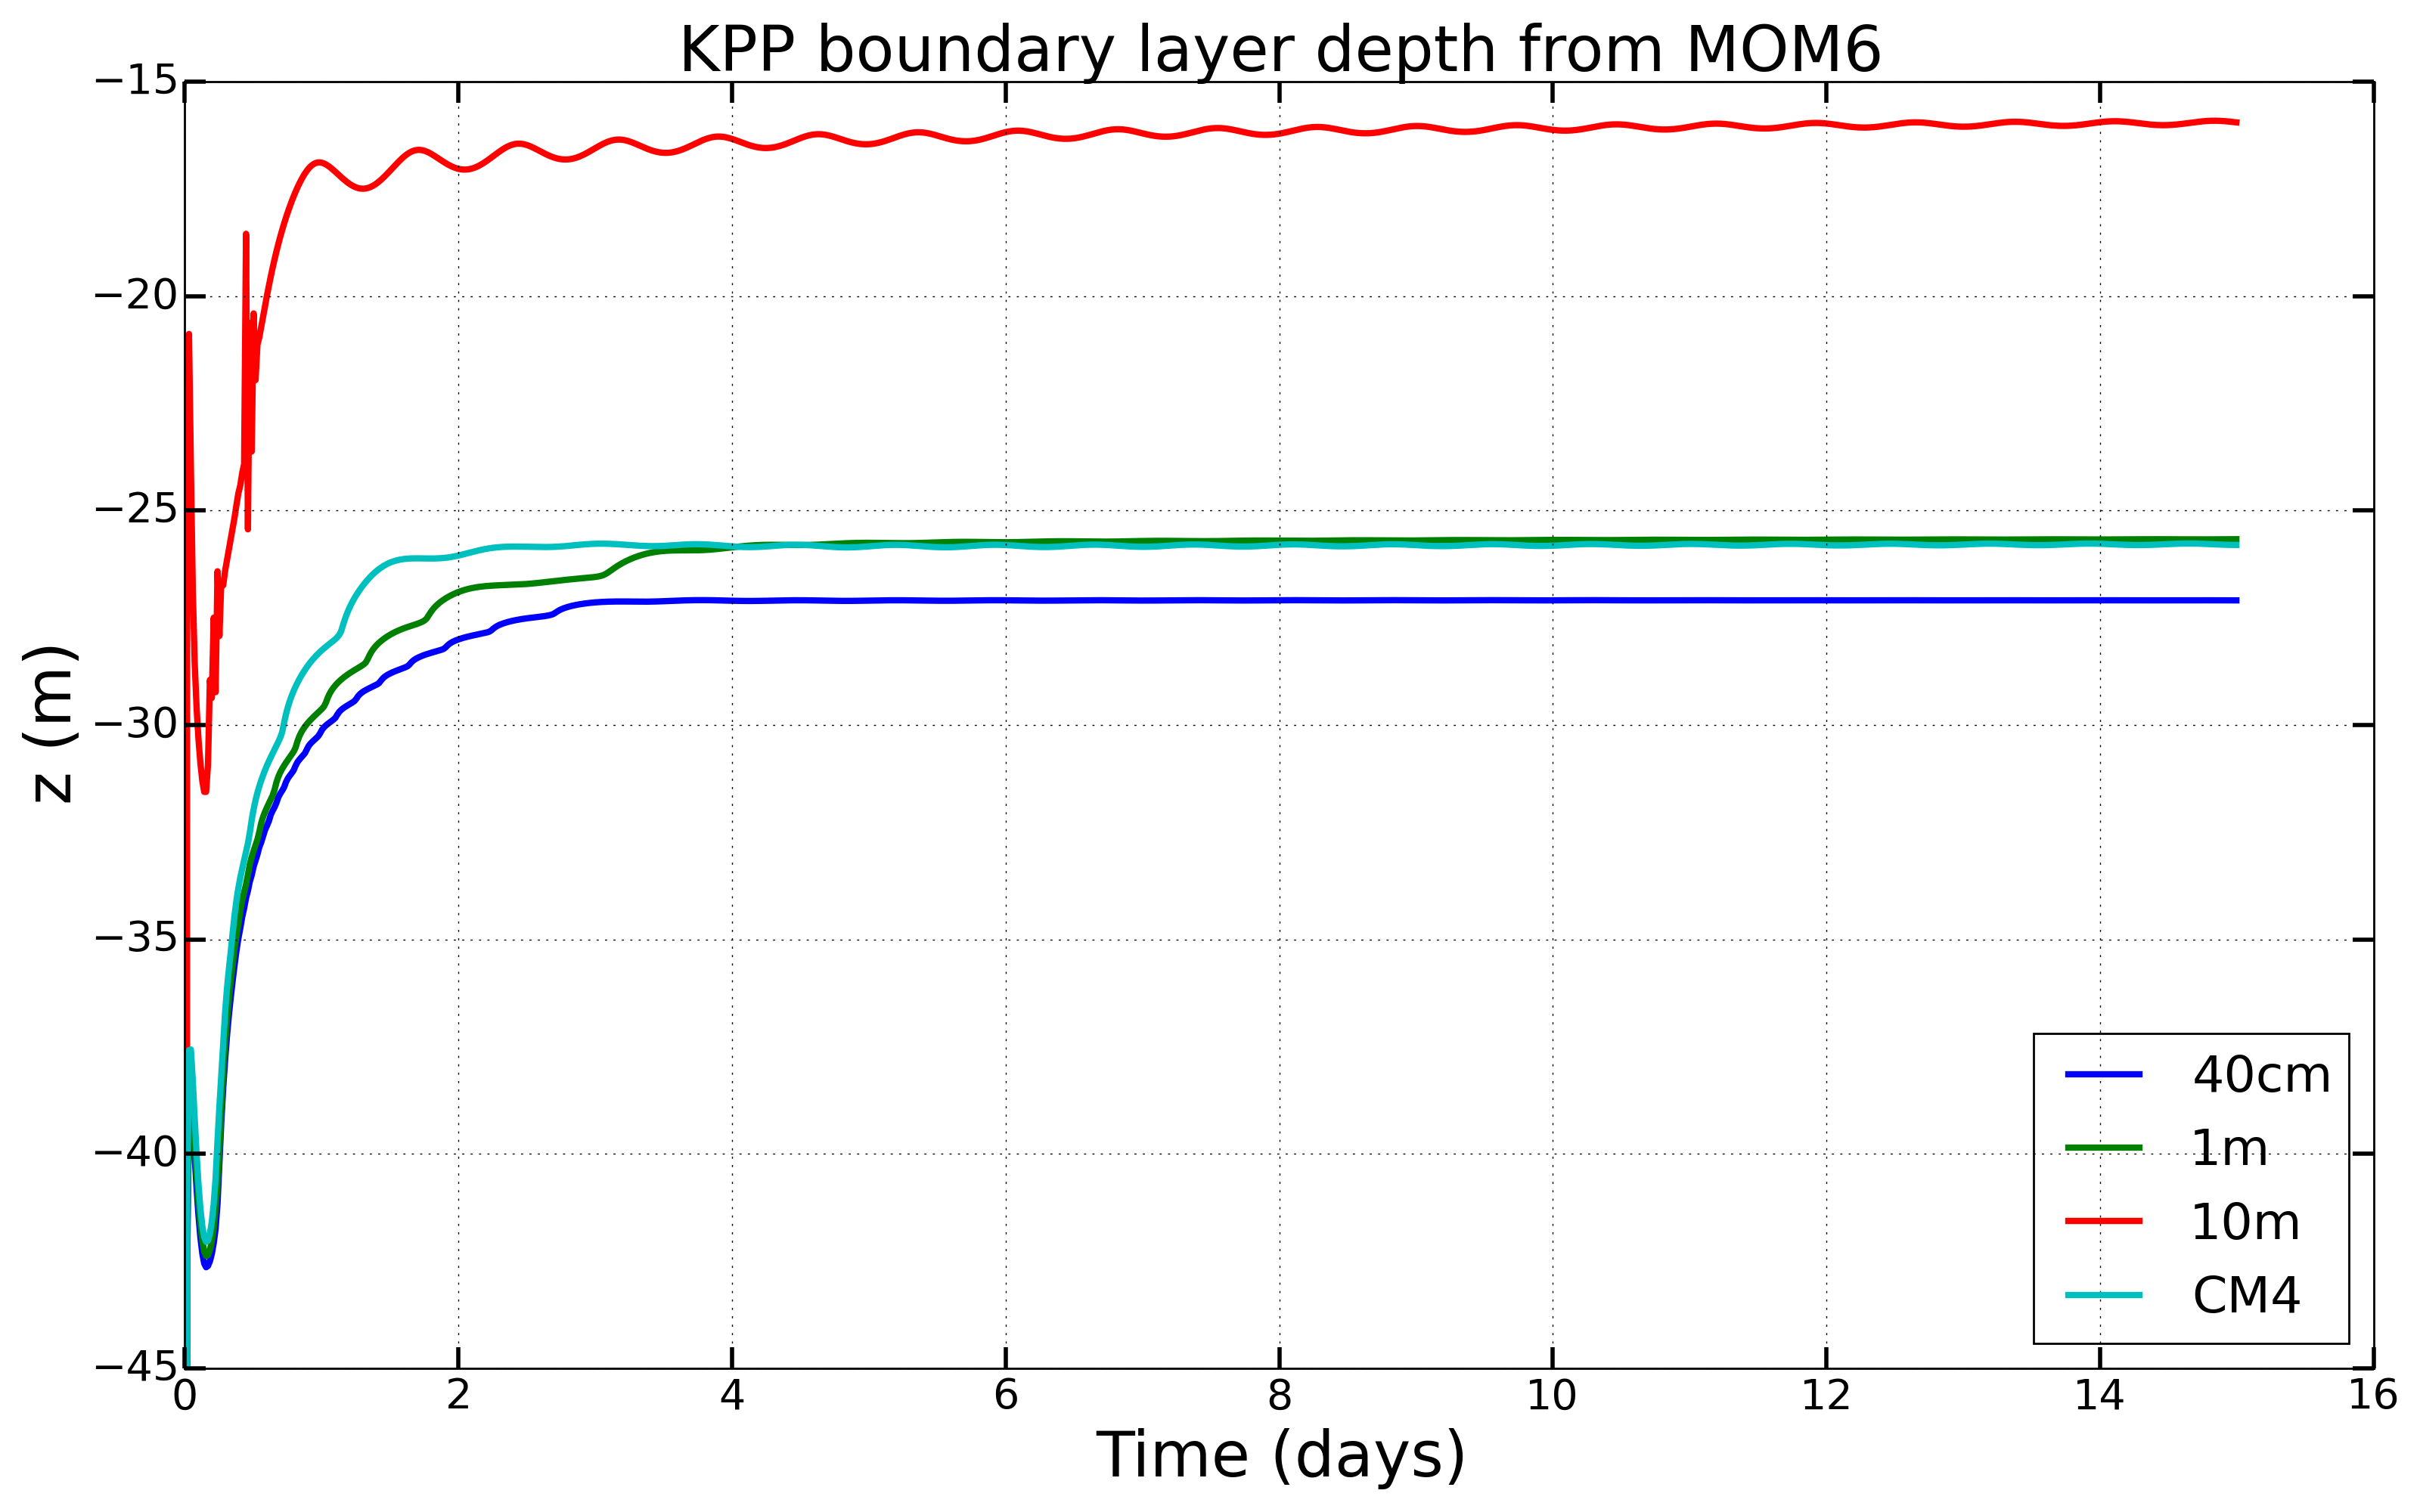
\includegraphics[angle=0,width=5cm]{./figs/MOM6/skin_warming_wind_KPP_MOM6_bldepth.png}
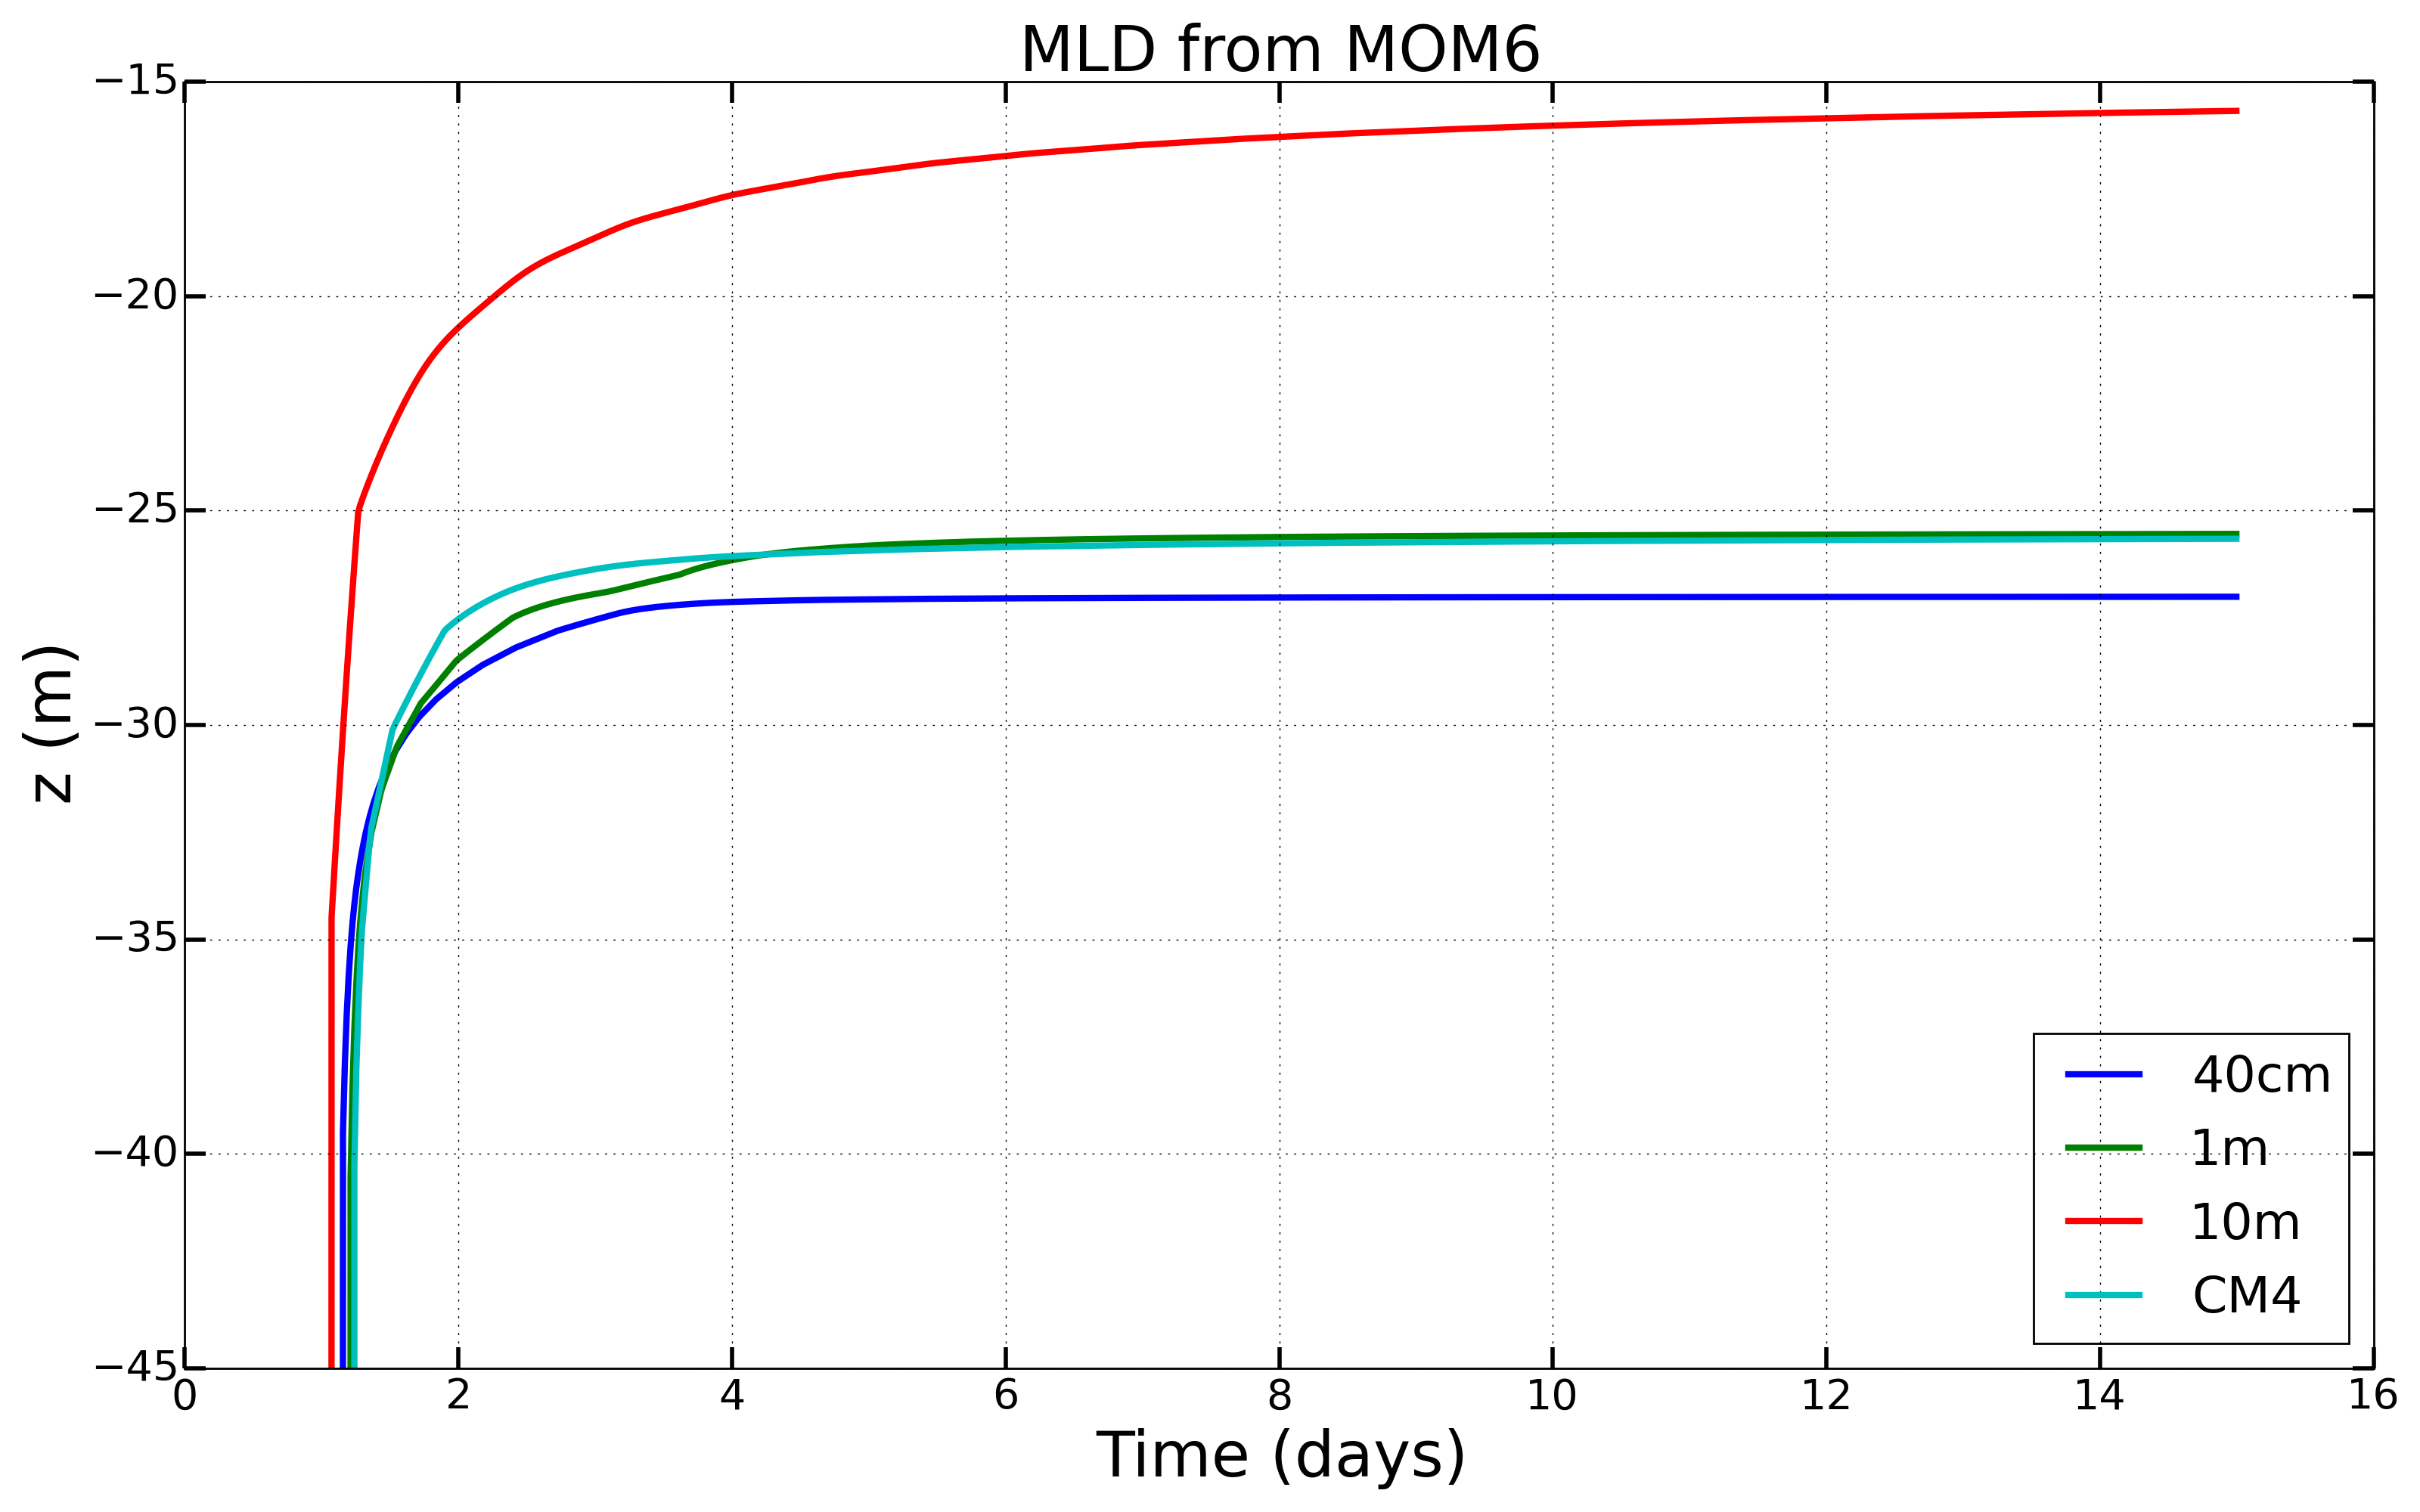
\includegraphics[angle=0,width=5cm]{./figs/MOM6/skin_warming_wind_KPP_MOM6_mld.png}
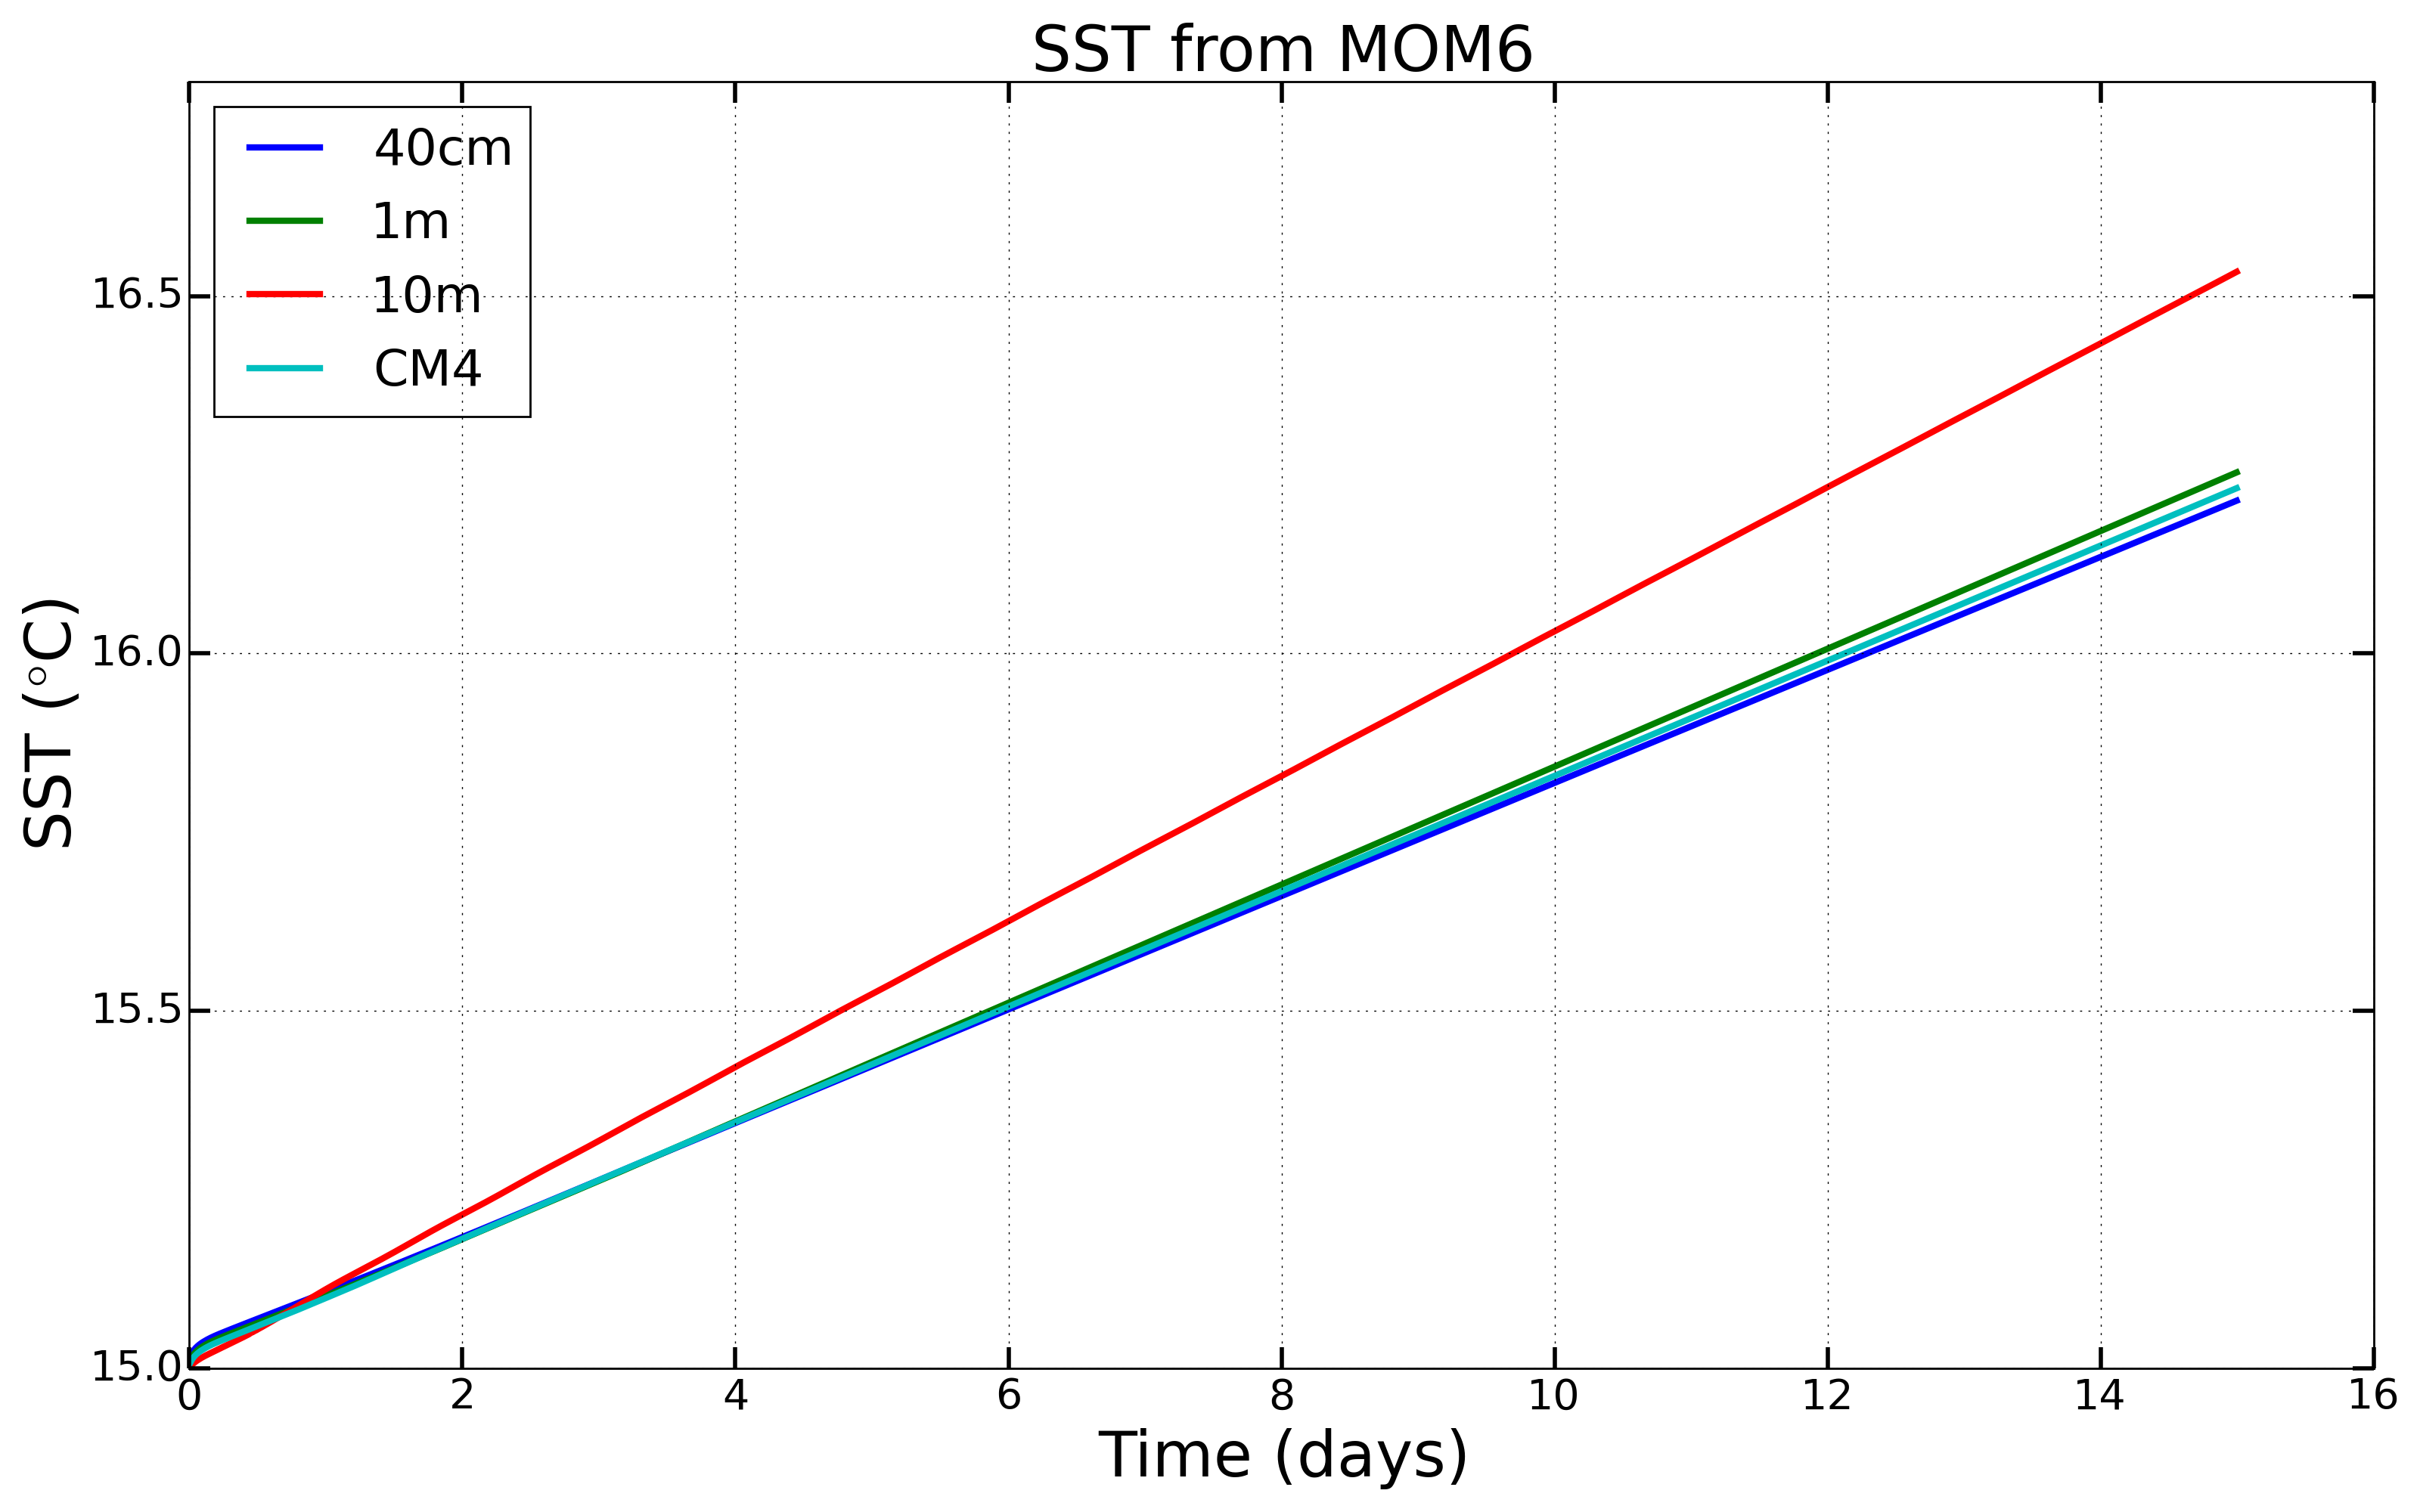
\includegraphics[angle=0,width=5cm]{./figs/MOM6/skin_warming_wind_KPP_MOM6_SST.png}
\caption[KPP BL depth, ML depth, and SST from MOM6 for warming+winds
test]{\sf Time series for KPP boundary layer depth (left panel), mixed
  layer depth (middle panel), and SST (right panel) for the
  warming+wind test case (constant zonal wind stress and
  $Q=100~\mbox{W}~\mbox{m}^{-2}$) as realized in MOM6.  The mixed
  layer depth is diagnosed as the depth where density differs from the
  surface by $0.003~\mbox{kg}~\mbox{m}^{-3}.$}
\label{fig:MOM6_SST_bldepth-wind_and_heating}
\end{center}
%\rule{\textwidth}{0.005in}
\end{figure}
%%%%%%%%%%%%%%%%%%%%%%%%%%%%%%%%%%%%%%%%%%%%%%%%%%%%%%%%%%%%%%%%%%%%%%%%


%%%%%%%%%%%%%%%%%%%% %%%%%%%%%%%%%%%%%%%%%%%%%
\begin{figure}[h!t]
%\rule{\textwidth}{0.005in}
\begin{center}
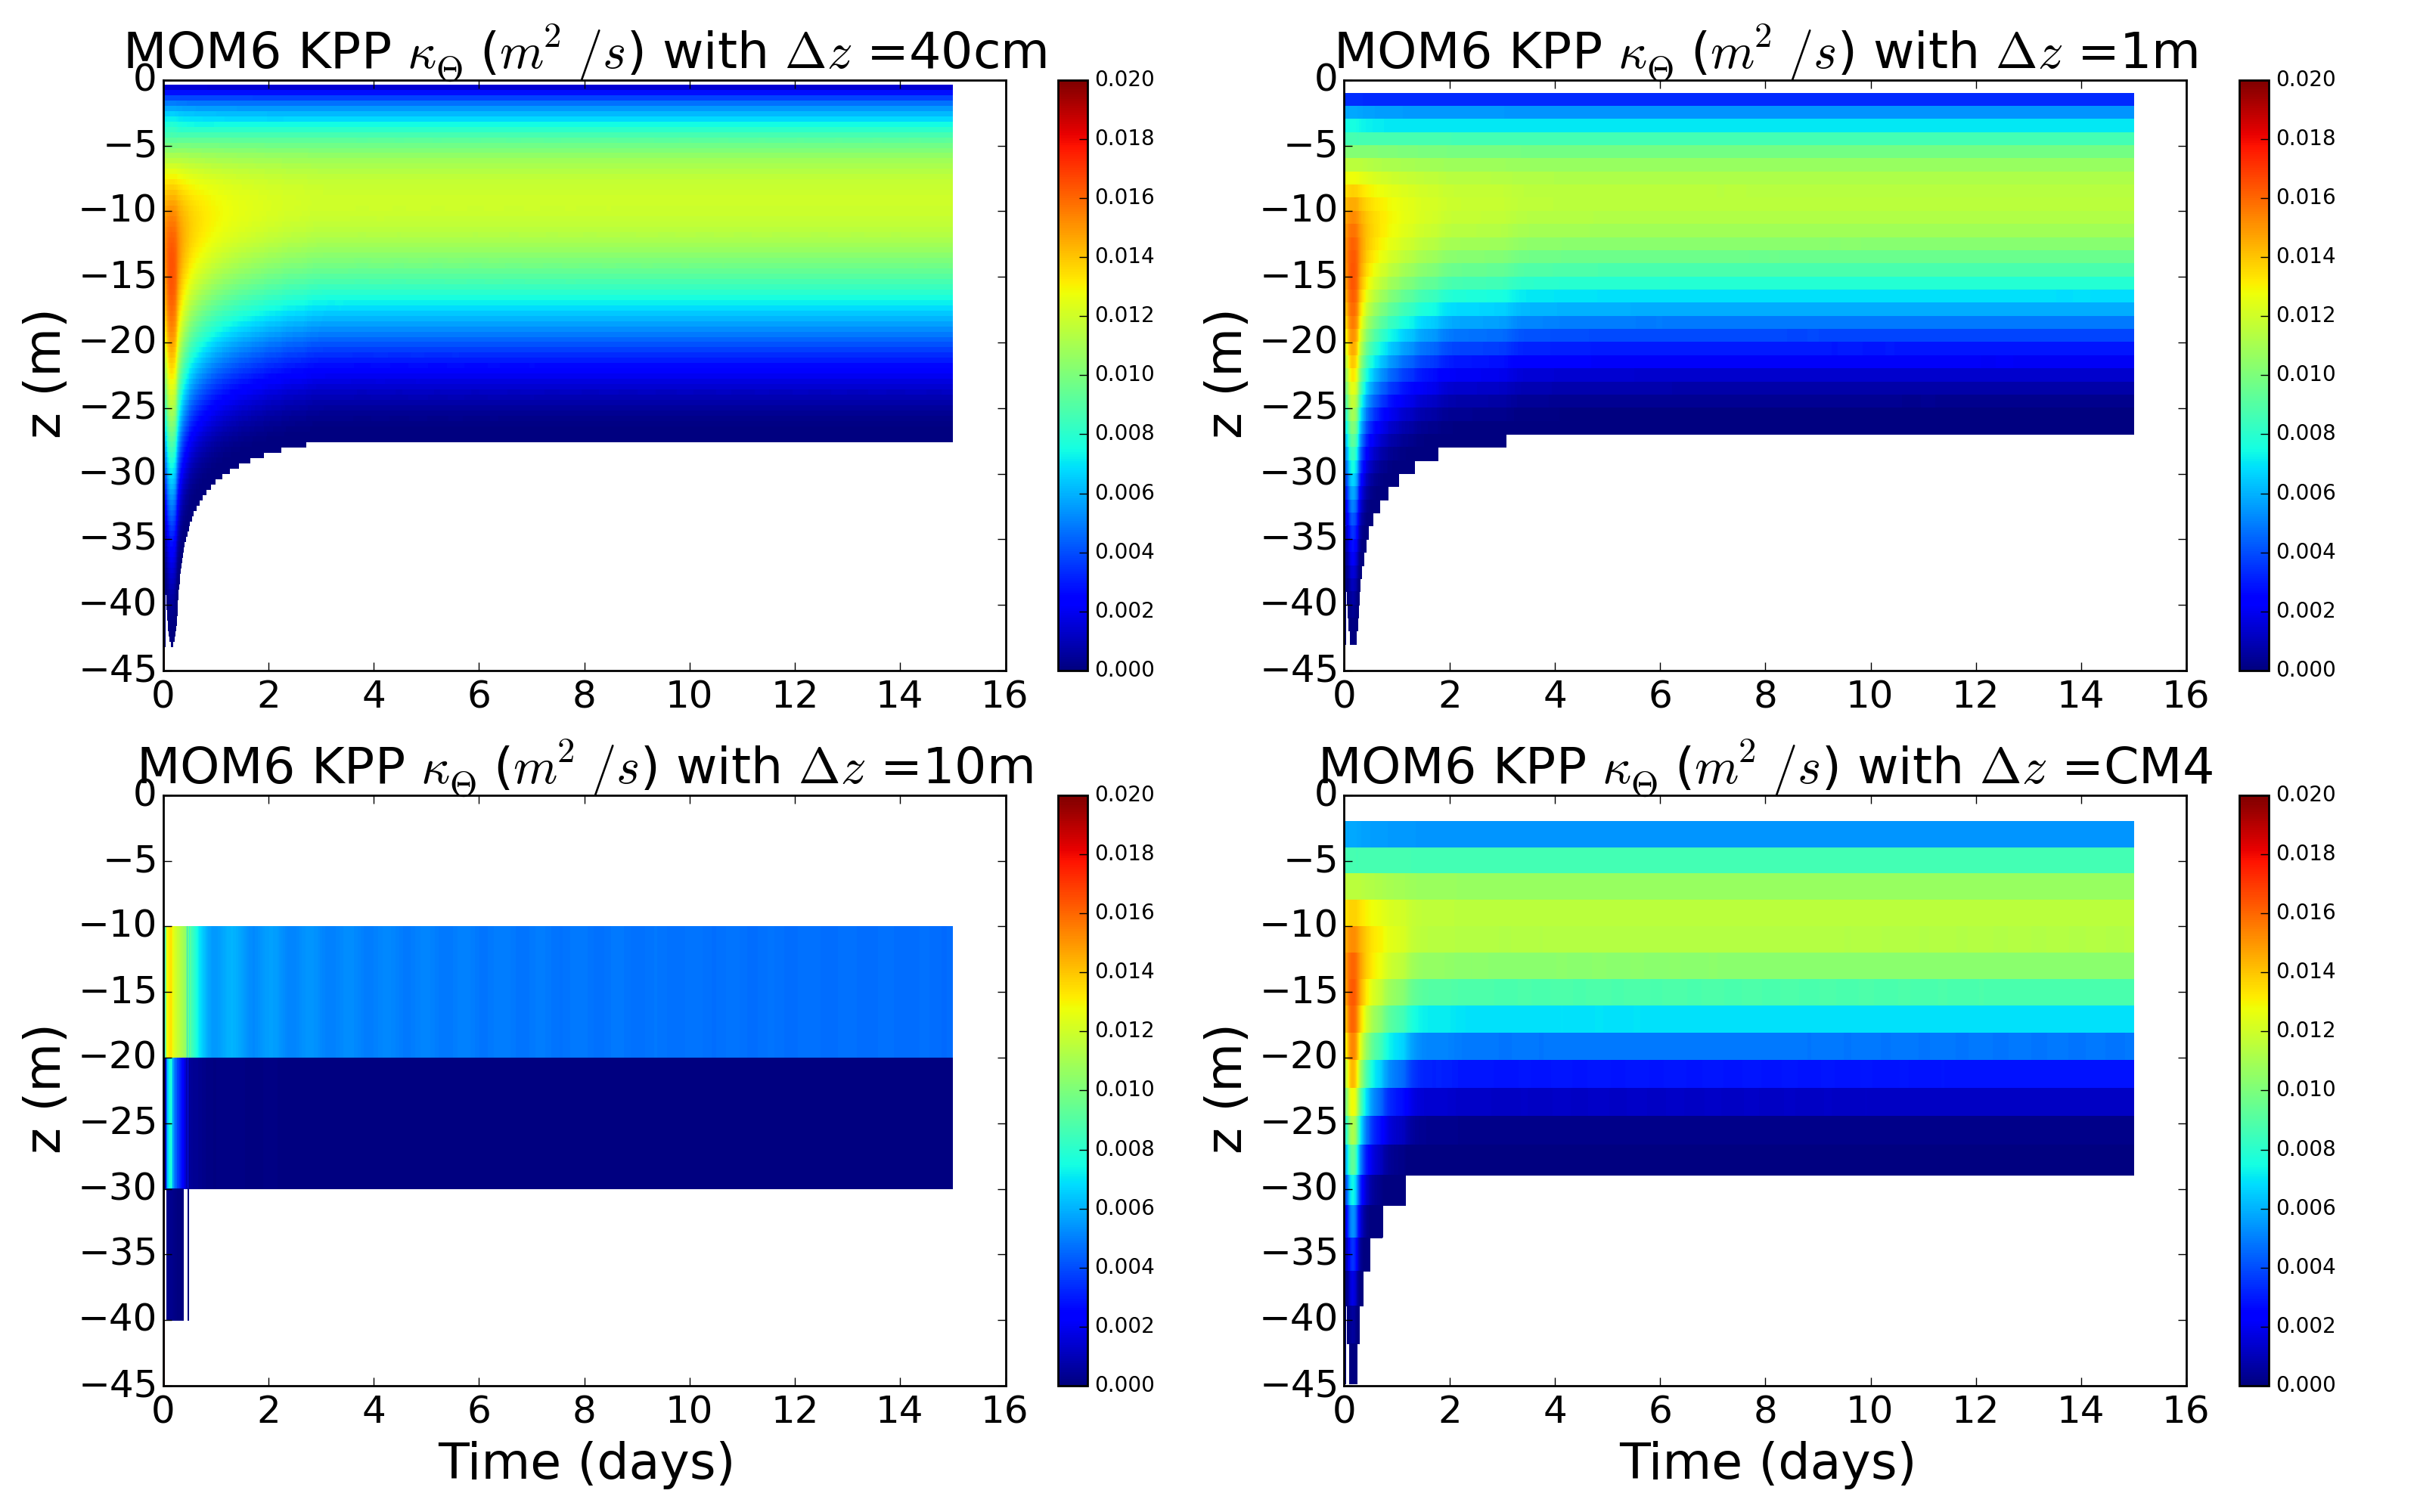
\includegraphics[angle=0,width=14cm]{./figs/MOM6/skin_warming_wind_KPP_MOM6_KPP_diffusivity.png}
\caption[KPP diffusivity from MOM6 for wind and heating test]{\sf Time
  series for the KPP vertical diffusivity for wind and heating test
  case (constant zonal wind stress and $Q=100~\mbox{W}~\mbox{m}^{-2}$)
  as realized in MOM6 using four different vertical grid resolutions.}
\label{fig:MOM6_KPP_diffusivity-wind_and_heating}
\end{center}
%\rule{\textwidth}{0.005in}
\end{figure}
%%%%%%%%%%%%%%%%%%%%%%%%%%%%%%%%%%%%%%%%%%%%%%%%%%%%%%%%%%%%%%%%%%%%%%%%


%%%%%%%%%%%%%%%%%%%% %%%%%%%%%%%%%%%%%%%%%%%%%
\begin{figure}[h!t]
%\rule{\textwidth}{0.005in}
\begin{center}
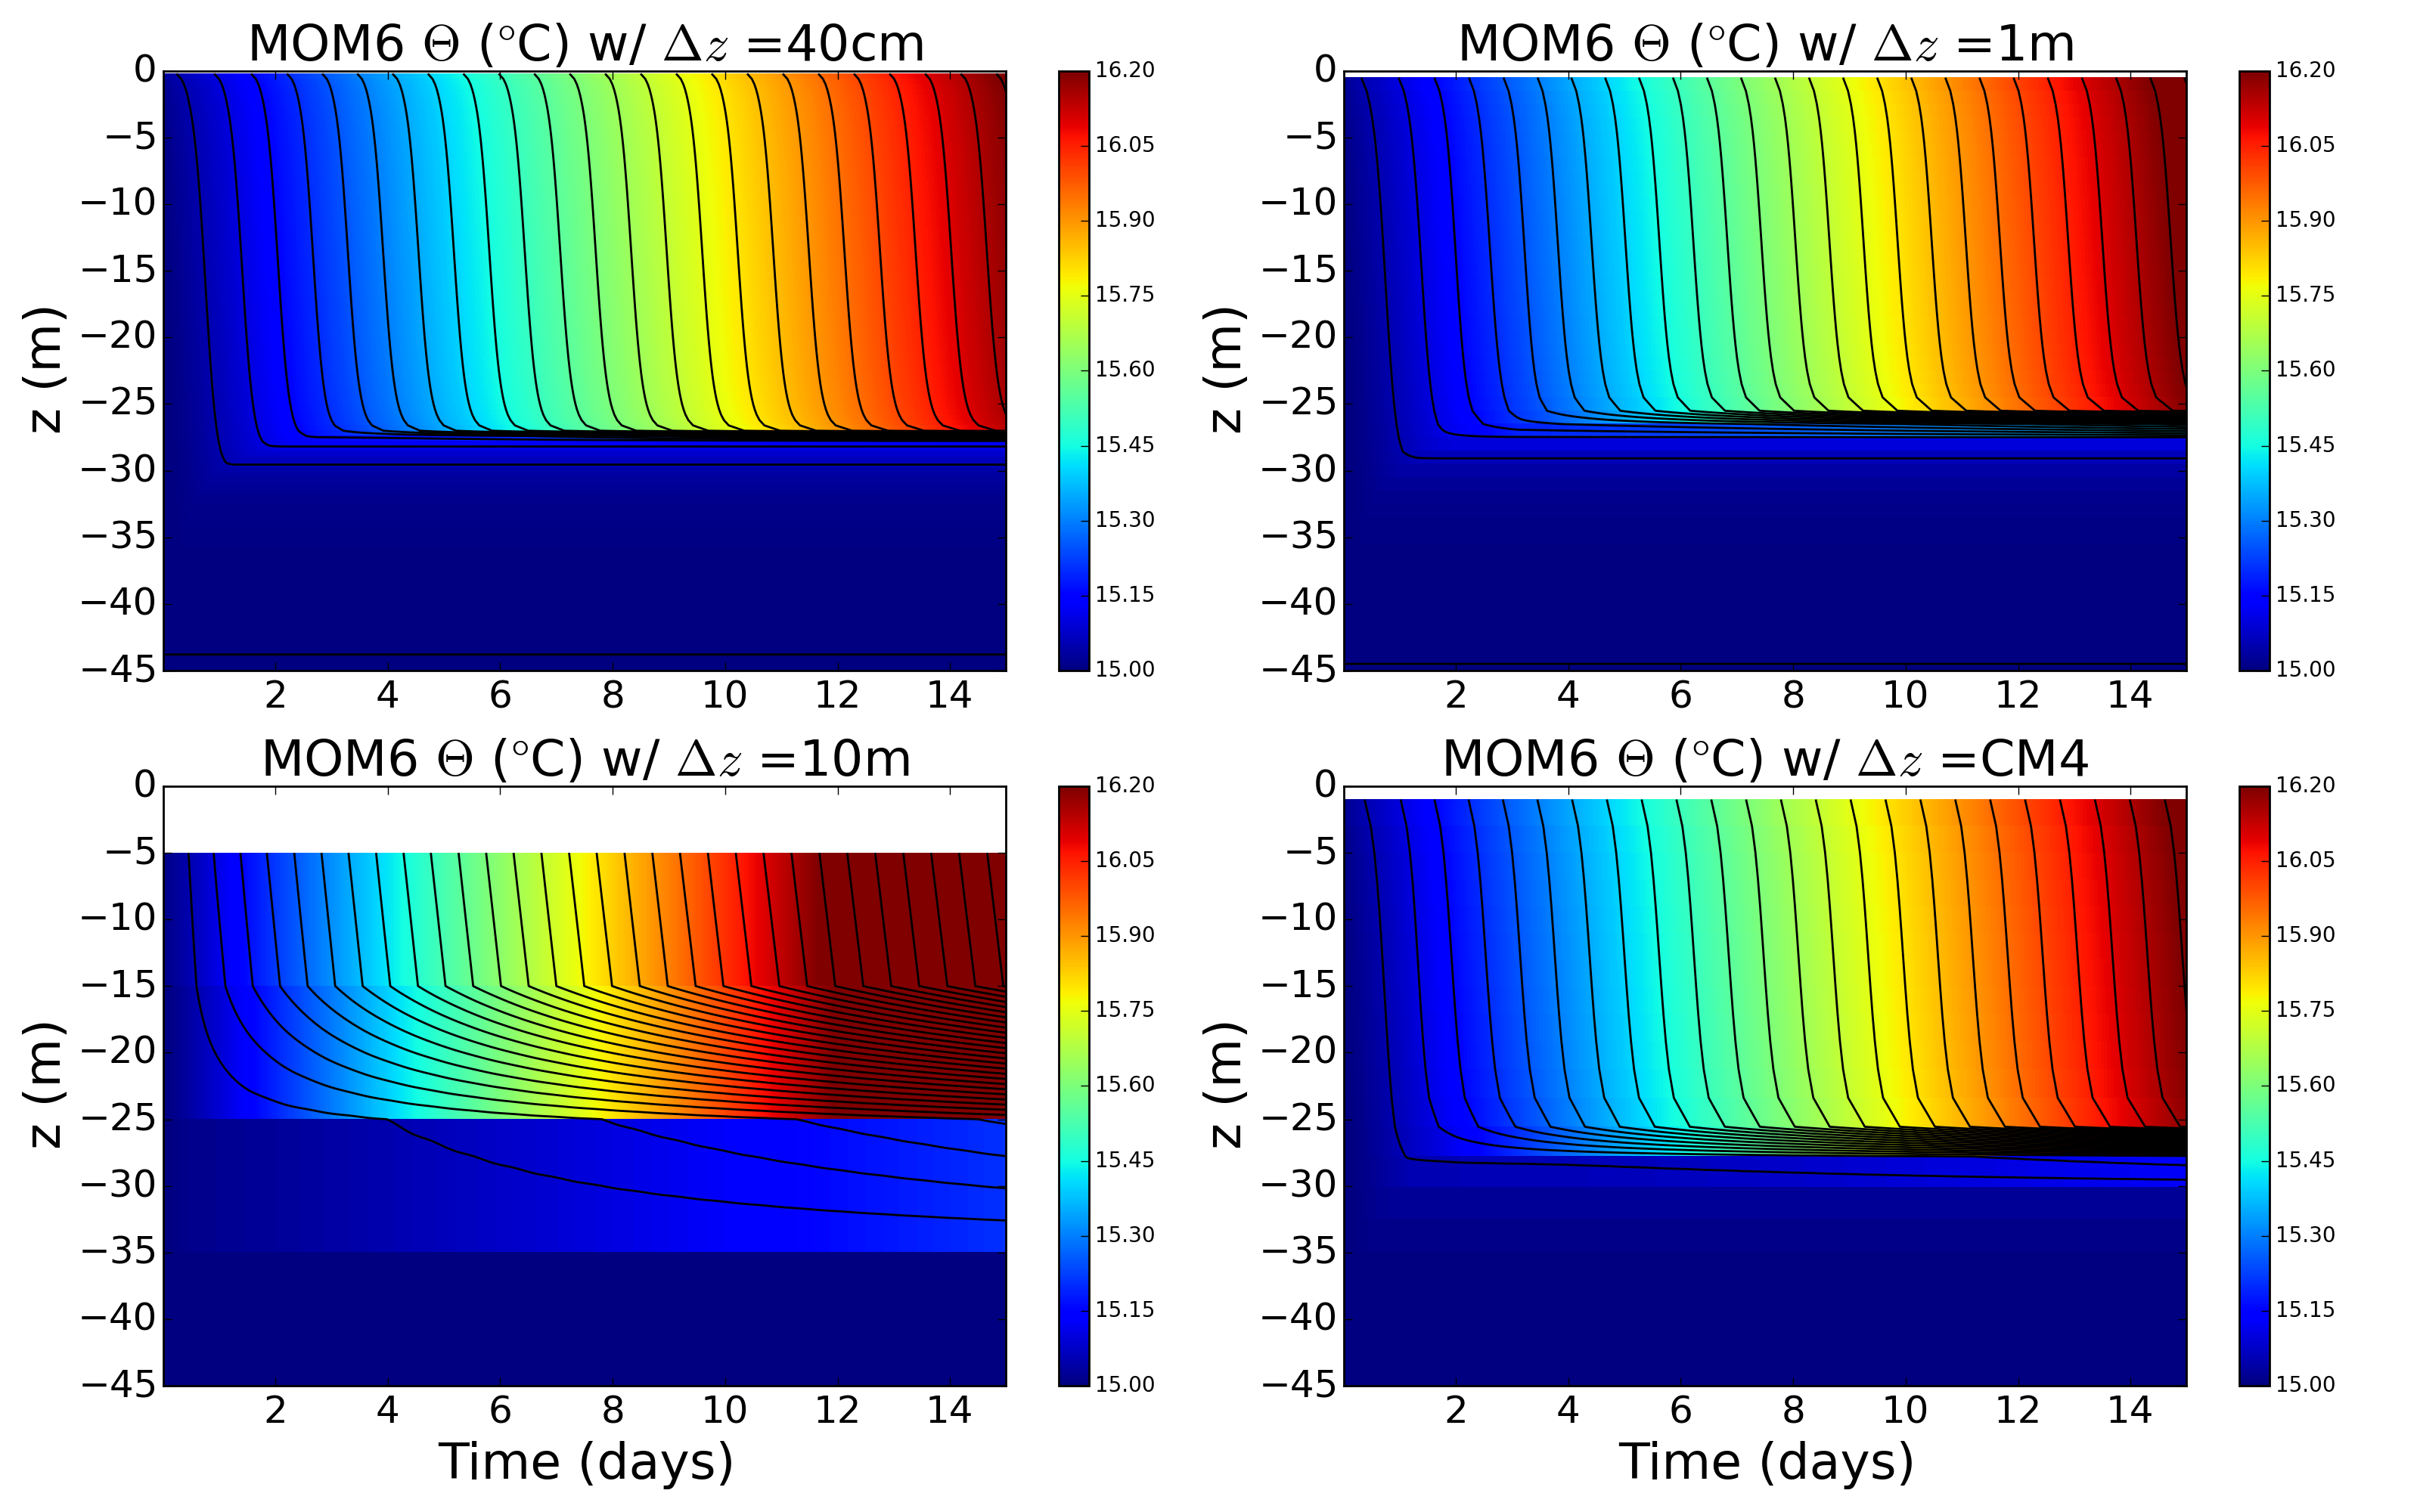
\includegraphics[angle=0,width=14cm]{./figs/MOM6/skin_warming_wind_KPP_MOM6_temp.png}
\caption[Temperature from MOM6 for wind and heating test]{\sf Time
  series for temperature from wind and heating test case (constant
  zonal wind stress and $Q=100~\mbox{W}~\mbox{m}^{-2}$) as realized in
  MOM6 using four different vertical grid resolutions.}
\label{fig:MOM6_temp-wind_and_heating}
\end{center}
%\rule{\textwidth}{0.005in}
\end{figure}
%%%%%%%%%%%%%%%%%%%%%%%%%%%%%%%%%%%%%%%%%%%%%%%%%%%%%%%%%%%%%%%%%%%%%%%%

%%%%%%%%%%%%%%%%%%%% %%%%%%%%%%%%%%%%%%%%%%%%%
\begin{figure}[h!t]
%\rule{\textwidth}{0.005in}
\begin{center}
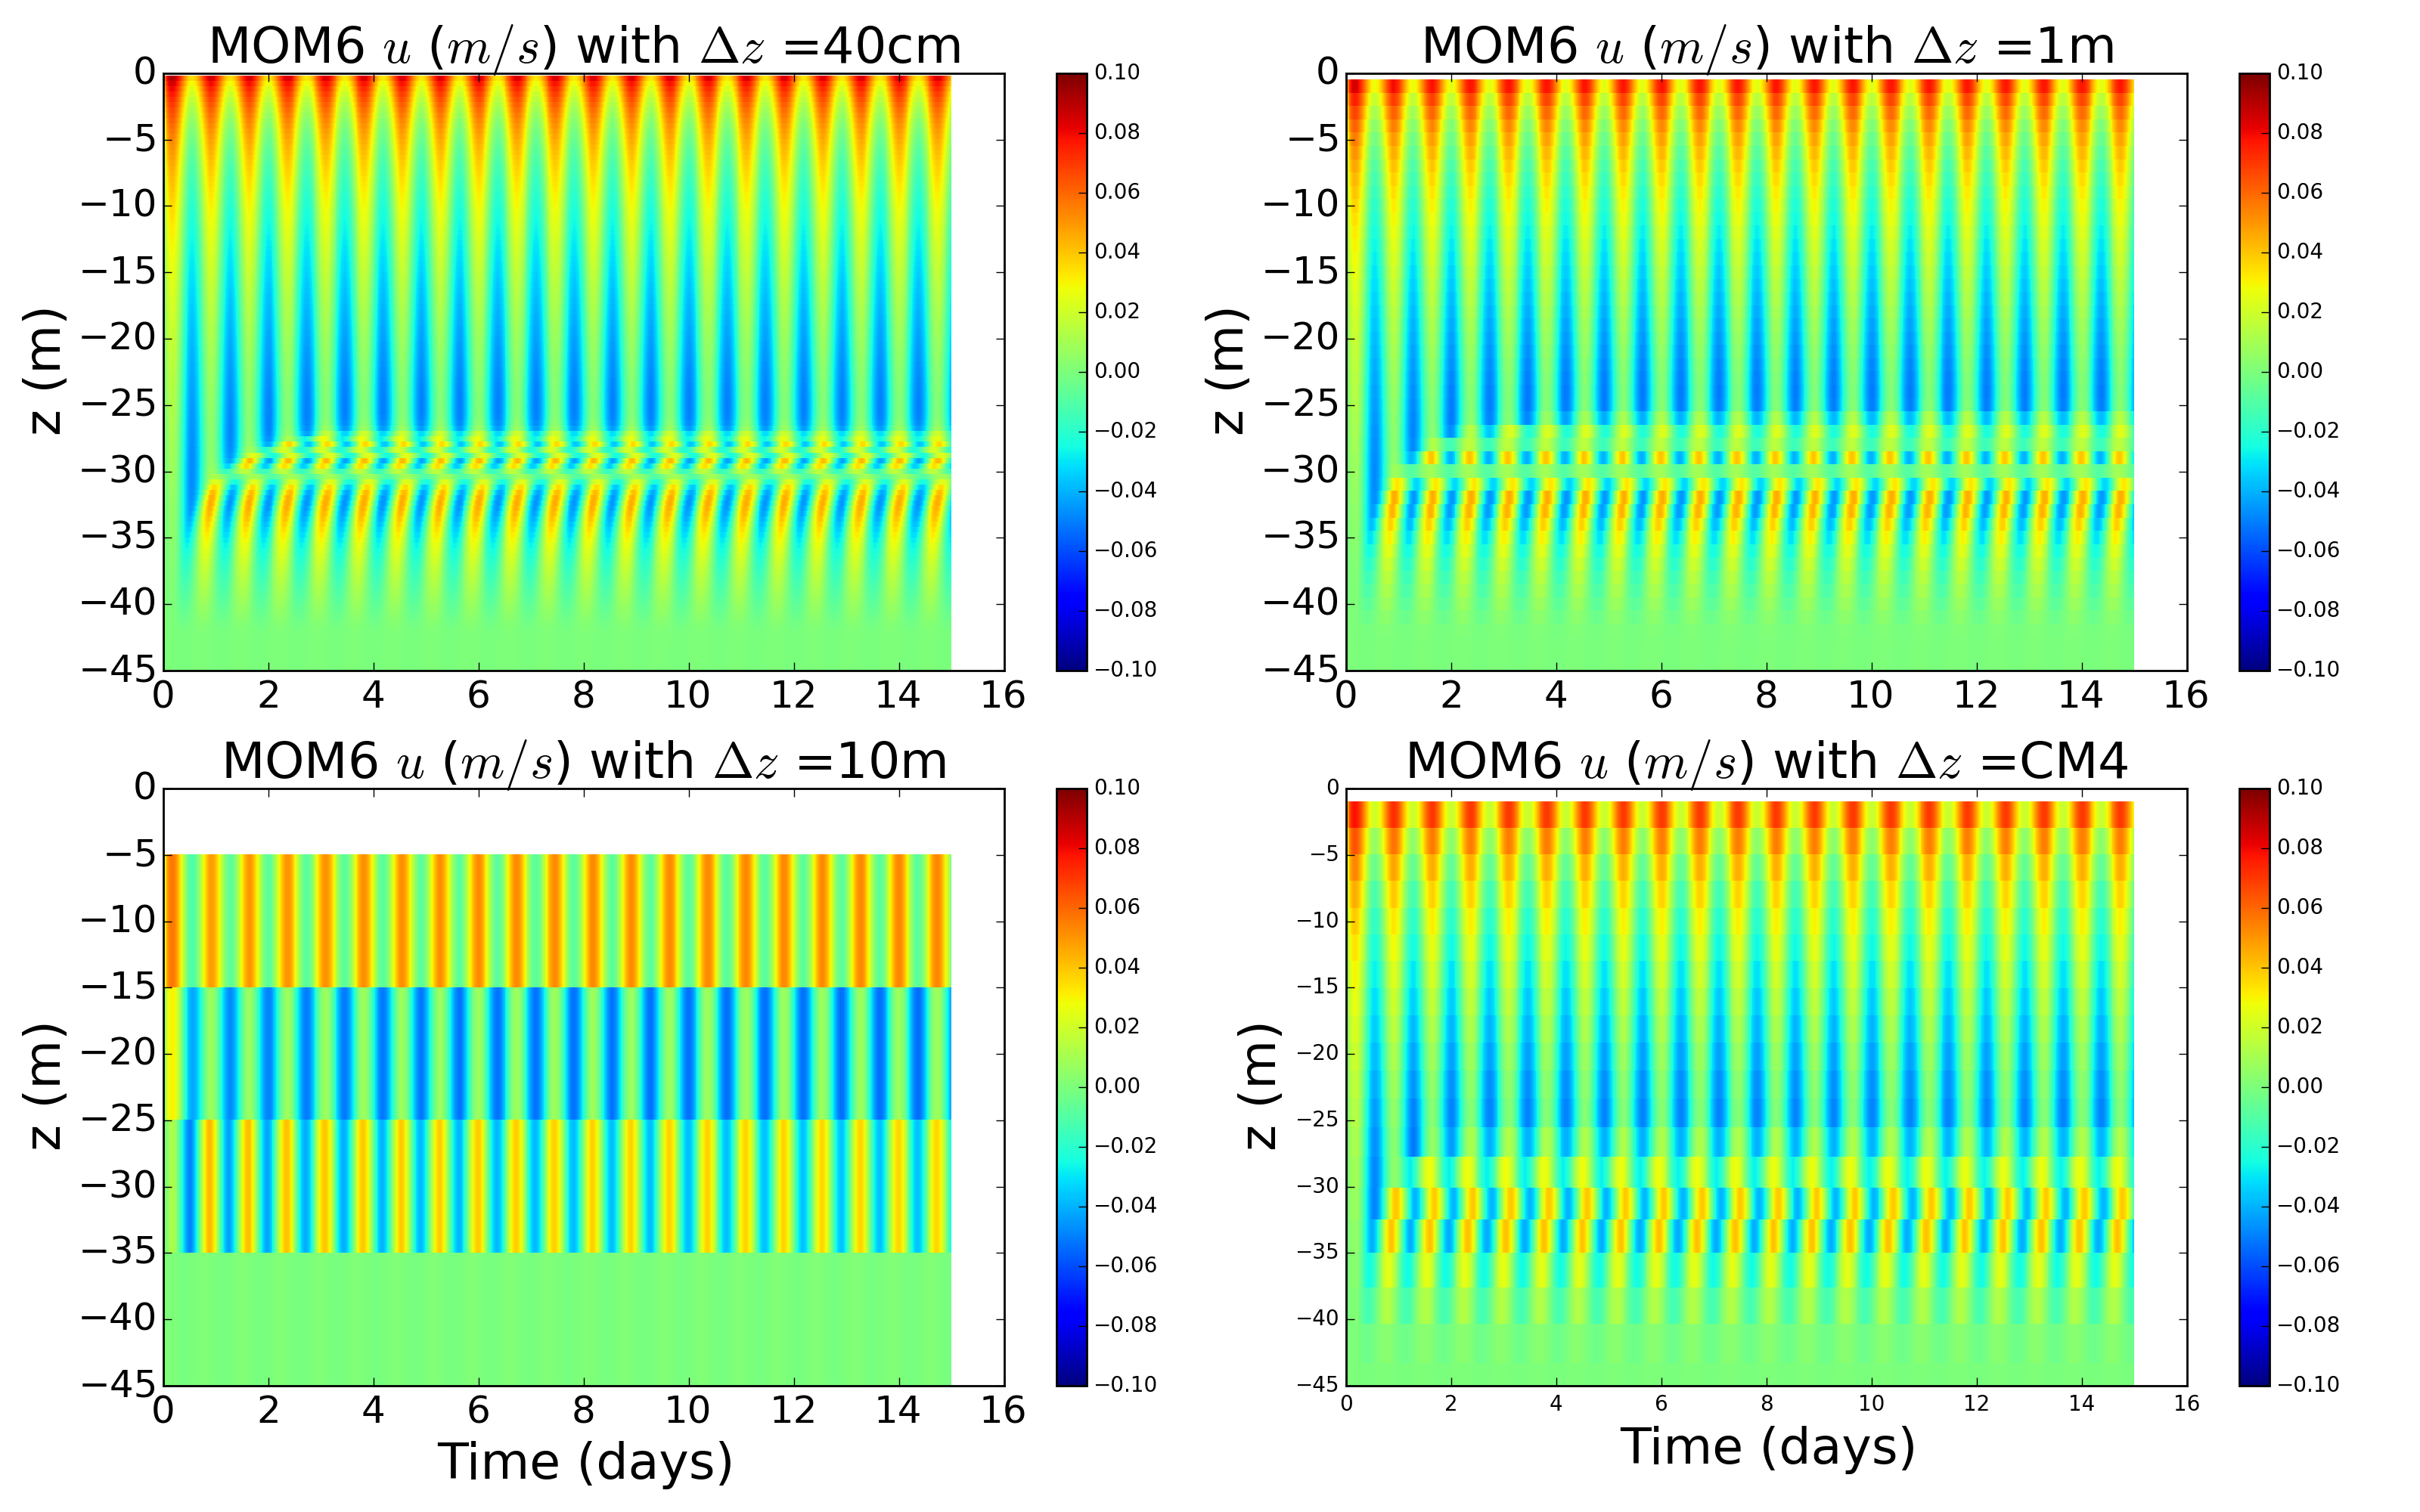
\includegraphics[angle=0,width=14cm]{./figs/MOM6/skin_warming_wind_KPP_MOM6_zonal_velocity.png}
\caption[Zonal velocity from MOM6 for wind and heating test]{\sf Time
  series for zonal velocity from wind and heating test case (constant
  zonal wind stress and $Q=100~\mbox{W}~\mbox{m}^{-2}$) as realized in
  MOM6 using four different vertical grid resolutions.}
\label{fig:MOM6_zonal-wind_and_heating}
\end{center}
%\rule{\textwidth}{0.005in}
\end{figure}
%%%%%%%%%%%%%%%%%%%%%%%%%%%%%%%%%%%%%%%%%%%%%%%%%%%%%%%%%%%%%%%%%%%%%%%%


